%% Version 4.3.2, 25 August 2014
%
%%%%%%%%%%%%%%%%%%%%%%%%%%%%%%%%%%%%%%%%%%%%%%%%%%%%%%%%%%%%%%%%%%%%%%
% Template.tex --  LaTeX-based template for submissions to the 
% American Meteorological Society
%
% Template developed by Amy Hendrickson, 2013, TeXnology Inc., 
% amyh@texnology.com, http://www.texnology.com
% following earlier work by Brian Papa, American Meteorological Society
%
% Email questions to latex@ametsoc.org.
%
%%%%%%%%%%%%%%%%%%%%%%%%%%%%%%%%%%%%%%%%%%%%%%%%%%%%%%%%%%%%%%%%%%%%%
%  PREAMBLE
%%%%%%%%%%%%%%%%%%%%%%%%%%%%%%%%%%%%%%%%%%%%%%%%%%%%%%%%%%%%%%%%%%%%%

%% Start with one of the following:
%  DOUBLE-SPACED VERSION FOR SUBMISSION TO THE AMS
\documentclass{ametsoc}

%  TWO-COLUMN JOURNAL PAGE LAYOUT---FOR AUTHOR USE ONLY
%\documentclass[twocol]{ametsoc}

\usepackage{multirow}
\usepackage{gensymb}

%%%%%%%%%%%%%%%%%%%%%%%%%%%%%%%%
%%% To be entered only if twocol option is used

\journal{jcli}

%  Please choose a journal abbreviation to use above from the following list:
% 
%   jamc     (Journal of Applied Meteorology and Climatology)
%   jtech     (Journal of Atmospheric and Oceanic Technology)
%   jhm      (Journal of Hydrometeorology)
%   jpo     (Journal of Physical Oceanography)
%   jas      (Journal of Atmospheric Sciences)	
%   jcli      (Journal of Climate)
%   mwr      (Monthly Weather Review)
%   wcas      (Weather, Climate, and Society)
%   waf       (Weather and Forecasting)
%   bams (Bulletin of the American Meteorological Society)
%   ei    (Earth Interactions)

%%%%%%%%%%%%%%%%%%%%%%%%%%%%%%%%
%Citations should be of the form ``author year''  not ``author, year''
\bibpunct{(}{)}{;}{a}{}{,}

%%%%%%%%%%%%%%%%%%%%%%%%%%%%%%%%

%%% To be entered by author:

%% May use \\ to break lines in title:

\title{Comparison of present reanalysis datasets in the context of the analogue method for statistical precipitation downscaling.}

%%% Enter authors' names, as you see in this example:
%%% Use \correspondingauthor{} and \thanks{Current Affiliation:...}
%%% immediately following the appropriate author.
%%%
%%% Note that the \correspondingauthor{} command is NECESSARY.
%%% The \thanks{} commands are OPTIONAL.

    %\authors{Author One\correspondingauthor{Author One, 
    % American Meteorological Society, 
    % 45 Beacon St., Boston, MA 02108.}
% and Author Two\thanks{Current affiliation: American Meteorological Society, 
    % 45 Beacon St., Boston, MA 02108.}}

\authors{Pascal Horton\correspondingauthor{University of Bern, Institute of Geography, Hallerstrasse 12, 3012 Bern, Switzerland.}, Rolf Weingartner, Stefan Br\"{o}nnimann}

%% Follow this form:
    % \affiliation{American Meteorological Society, 
    % Boston, Massachusetts.}

\affiliation{Oeschger Centre for Climate Change Research, Institute of Geography, University of Bern, Bern, Switzerland}

%% Follow this form:
    %\email{latex@ametsoc.org}

\email{pascal.horton@giub.unibe.ch}

%% If appropriate, add additional authors, different affiliations:
    %\extraauthor{Extra Author}
    %\extraaffil{Affiliation, City, State/Province, Country}

\extraauthor{Charles Obled}
\extraaffil{Institut des G\'{e}osciences de l'Environnement, Universit\'{e} de Grenoble-Alpes, Grenoble, France}


%%%%%%%%%%%%%%%%%%%%%%%%%%%%%%%%%%%%%%%%%%%%%%%%%%%%%%%%%%%%%%%%%%%%%
%  ABSTRACT
%
% Enter your abstract here
% Abstracts should not exceed 250 words in length!
%
% For BAMS authors only: If your article requires a Capsule Summary, please place the capsule text at the end of your abstract
% and identify it as the capsule. Example: This is the end of the abstract. (Capsule Summary) This is the capsule summary. 

\abstract{
	%The analogue method is a statistical downscaling method for precipitation prediction. It uses similarity in terms of synoptic-scale predictors with situations in the past in order to provide a probabilistic prediction for the day of interest. It has been used for decades in a context of weather or flood forecasting, and is more recently also applied to climate studies, whether for reconstruction of past weather conditions or future climate impact studies. In order to evaluate the relationship between synoptic scale predictors and the local weather variable of interest, e.g. precipitation, reanalysis datasets are necessary. Nowadays, the number of available reanalysis datasets increase. These are generated by different atmospheric models with different assimilation techniques and offer various spatial and temporal resolutions. A major difference between these datasets is also the length of the archive they provide. While some datasets start at the beginning of the satellite era and assimilate these data, others aim at homogeneity on a longer period and only assimilate conventional observations.
%The context of the application of analogue methods might drive the choice of an appropriate dataset, for example when the archive length is a leading criterion. However, in many studies, a reanalysis dataset is subjectively chosen, according to the user’s preferences or the ease of access. The impact of this choice on the results of the downscaling procedure is rarely considered and no comprehensive comparison has been undertaken so far.
%In order to fill this gap and to advise on the choice of appropriate datasets, nine different global reanalysis datasets were compared in seven distinct versions of analogue methods, over 300 precipitation stations in Switzerland. Significant differences in terms of prediction performance were identified. Although the impact of the reanalysis dataset on the skill score varies according to the chosen predictor, be it atmospheric circulation or thermodynamic variables, some hierarchy between the datasets is often preserved.
}

\begin{document}

%% Necessary!
\maketitle


%%%%%%%%%%%%%%%%%%%%%%%%%%%%%%%%%%%%%%%%%%%%%%%%%%%%%%%%%%%%%%%%%%%%%
%  MAIN BODY OF PAPER
%%%%%%%%%%%%%%%%%%%%%%%%%%%%%%%%%%%%%%%%%%%%%%%%%%%%%%%%%%%%%%%%%%%%%
%

%% In all cases, if there is only one entry of this type within
%% the higher level heading, use the star form: 
%%
% \section{Section title}
% \subsection*{subsection}
% text...
% \section{Section title}

%vs

% \section{Section title}
% \subsection{subsection one}
% text...
% \subsection{subsection two}
% \section{Section title}

%%%
% \section{First primary heading}

% \subsection{First secondary heading}

% \subsubsection{First tertiary heading}

% \paragraph{First quaternary heading}


%TODO: publish results as datasets?
%TODO: AM not sensitive to biases

\section{Introduction}

Reanalysis datasets have a wide range of application. Among these are statistical downscaling methods, which use these global gridded data as predictors in order to predict a local variable of interest, such as precipitation. The present work focuses on the analogue method (AM), which is a statistical downscaling technique relying on the hypothesis that similar synoptic situations are likely to result in similar local effect, plus a certain variability that is not explained by the considered predictors. In order to take into account this unertainty, several analogue days are extracted from the archive and provide the empirical conditional distribution that is the statistical prediction for the considered target day. Different versions of AMs exist, relying on various predictors. 

In former time, the predictors of the AM were extracted from radio-sounding data \citep{Duband1981}, which involved heavy pre-treatment to have a complete and homogeneous database that can be used. The release of the first reanalysis dataset \citep[NCEP/NCAR Reanalysis I, NR-1][]{Kalnay1996, Kistler2001} greatly simplified the implementation of the AM, and opened new opportunities of using other variables. \citet{Bontron2004} assessed most variables of the NR-1 dataset to end up with two methods: one based on the atmospheric circulation and the second one adding a second level of analogy on moisture variables.



The goal of this work is to quantify the impact of choosing a certain reanalysis dataset for the AM, and to analyze the role of the dataset resolution. Additionnally, the role of the archive size will be discussed, along with the use of different members of datasets providing ensembles.


"Reanalysis data provide a multivariate, spatially complete, and coherent record of the global atmospheric circulation" \cite{Dee2011a} "produced with a single version of a data assimilation system –including the forecast model used –and is therefore not affected by changes in method"
"The accuracy of these model-generated estimates naturally depends on the quality of the model physics aswell asthat of the analysis. "\cite{Dee2011a}

\section{Data and methods}
\label{sec:data}

\subsection{Reanalysis datasets}

The considered global atmospheric reanalysis datasets are briefly described hereafter and some of their characteristics are provided in Table \ref{table:datasets}. The common period to all datasets is 1981--2010. All reanalysis products are available at a 6-h time step, with some datasets or variables having higher temporal resolution. Only the 6-h time step is considered in the present work.

\subsubsection{NCEP Reanalysis I}

The NCEP/NCAR Reanalysis I \citep[NR-1,][]{Kalnay1996, Kistler2001} is the first global reanalysis product. It was made with a model frozen at the state-of-the-art of 1995 and by assimilating land surface, ship, aircraft, rawinsonde, and satellite data among others, after quality control. However, upper-air observations have a much larger influence on the analysis than the surface observations \citep{Kistler2001}. The data assimilation system is a 3D variational technique (3D-Var). The model resolution is T62 (about 210~km) with 28 sigma vertical levels. All major physical processes are parameterized. The period coverage was starting first in 1957, before being extended to 1948. \citet{Kalnay1996} were aware that assimilating all available data at a give time would have impact on the climate of the reanalysis due to changes in the observating system, but the choice was made for accuracy over stability of the climate. A comparison of two sets of analyses made with and without the use of satellite data showed that even without satellite data, almost 100\% of the daily variance of the geopotential height was explained in the NH extratropics \citep{Kalnay1996}. Lower correlation values were found in other regions of the globe, particularly in the Southern Hemisphere, where the uncertainty is much higher due to the lack of rawinsonde data. However, rms of the analysis increments (difference between the forecast and the analysis) at 500~hPa showed large differences between a data-poor year (1958) and a data-rich year (1996), and the climatologies before and after 1979 differ significantly due to the use of satellite data \citep{Kistler2001}.


\subsubsection{NCEP Reanalysis II}

The NCEP–DOE Reanalysis 2 \citep[NR-2,][]{Kanamitsu2002} is a follow-on to the NCEP/NCAR Reanalysis I project with the goal to correct known problems that were identified after the NR-1 production, mainly human processing errors. However. these issues have consequences for a limited number of applications. NR-2 also relies on updated versions of the assimilation system and the model, with improvements to the model physics. Changes in parameterizations have improved the precipitation estimate, but may have caused deterioration of other variables \citep{Kistler2001, Kanamitsu2002}. Primary analysis variables, such as geopotential heights, only contains minor differences with NR-1.

The model and the outputs have the same spatial and temporal resolution as NR-1, and it relies on mostly the same observational data.


\subsubsection{ERA-Interim}

ERA-Interim \citep[ERA-INT, ][]{Dee2011a} is produced by the European Centre for Medium-Range Weather Forecasts (ECMWF) and covers the period from 1979 onwards. It replaced ERA-40 \citep{Uppala2005}, which replaced ERA-15 \citep{Gibson1997}, reanalysis datasets of 45 and 15 years respectively. ERA-INT aims at addressing problems in data assimilation of ERA-40 and at improving several technical aspects in the process, which are expected to have an impact on the quality of the product.

ERA-INT uses a 4D variational technique (4D-Var) with sequential data assimilation in 12-hourly analysis cycles. It assimilates conventional observations, rawinsonde, aircraft, and satellite data, etc. 4D-Var is expected to make a more effective use of observations \citep{Dee2011a}. ERA-INT also relies on several bias and error correction techniques that were introduced after ERA-40 in order to minimise inconsistencies between observations of different types.

The atmospheric model uses a hybrid sigma-pressure vertical coordinate on 60 layers and has a T255 horizontal resolution (about 79~km) and a 30~min time step. Orographic effects and convection schemes, among others, have been improved since ERA-40.


\subsubsection{Climate Forecast System Reanalysis}

The Climate Forecast System Reanalysis \citep[CFSR, ][]{Saha2010a} is the second generation of global reanalyses provided by NCEP. The model resolution was significantly increased since NR-1/NR-2 : horizontal resolution of T382 (about 38~km) and 64 vertical levels on sigma-pressure hybrid vertical coordinates. Both the model and the assimilation were also improved. New parameterizations were used, resulting in more realistic moisture prediciton and mountain blocking representation, among others \citep{Saha2010a}. There is also a coupling to the ocean and a sea ice model.

The assimilation scheme relies on the 3D-Var technique, but with a certain consideration of the time aspect by using time tendencies of state variables. The assimilated data are most of available observations from different kind of sensors, selected after quality control. The period covered is from 1979 onwards, but the initial plan was to extend it back to 1947 or earlier \citep{Saha2010a}.

"Another notable difference between R1 and/or
R2 and the CFSR is that the CFSR GSI uses satellite radiances rather than derived temperature or mois- ture profiles. This allows the GSI greater freedom to generate adjustments to the temperature, moisture, and ozone fields to best match the observed radiances."


CFSR has the particularity to analyze the historical tropical storm locations. The substantial benefit is that "by relocating a tropical storm vortex to its observed location prior to the assimilation of storm circulation observations, distortion of the circulation by the mismatch of guess and observed locations is avoided" \citep{Saha2010a}.



"It is worth noting that the analysis system used in CFSR for the atmosphere, the GSI scheme, is nearly the same as the one used by MERRA at the NASA GSFC"
Gridded statistical interpolation
"The MERRA atmosphere-only reanalysis is being conducted over the same years with nearly the same input data."

\subsubsection{Japanese 55-year Reanalysis}

JRA-55 \citep{Kobayashi2015, Harada2016}
JRA-55C


The first global reanalysis to assimilate historical tropical storm information was JRA-25 (Onogi et al.
2007).

\subsubsection{NOAA-CIRES 20th Century Reanalysis}

20CR-2c \citep{Compo2011}





\subsubsection{ECMWF 20th Century Reanalysis}

ERA-20C \citep{Poli2016}





\subsubsection{MERRA-2}

\cite{Gelaro2017}
MERRA-2. MERRA-2 is an update for the first MERRA reanalysis \citep{Rienecker2011}





\subsubsection{ECMWF Coupled 20th Century Reanalysis}

CERA-20C






%https://www.ncbi.nlm.nih.gov/pmc/articles/PMC4461156/
%http://reanalyses.org/comment/3843
%https://disc.gsfc.nasa.gov/datareleases/merra_2_data_release
%https://climatedataguide.ucar.edu/climate-data/era-20c-ecmwfs-atmospheric-reanalysis-20th-century-and-comparisons-noaas-20cr?qt-climatedatasetmaintabs=5#qt-climatedatasetmaintabs
%https://climatedataguide.ucar.edu/climate-data/era-20c-ecmwfs-atmospheric-reanalysis-20th-century-and-comparisons-noaas-20cr
%https://www.esrl.noaa.gov/psd/data/gridded/data.ncep.reanalysis.derived.html
%https://www.esrl.noaa.gov/psd/data/20thC_Rean/
%https://climatedataguide.ucar.edu/climate-data/atmospheric-reanalysis-overview-comparison-tables



\subsection{Precipitation dataset}
\label{sec:precip}

The predictands -- variables to be predicted -- considered here are daily precipitation totals (06:00 h UTC to 06:00 h UTC the following day) at 301 weather stations of the MeteoSwiss network in Switzerland (Fig. \ref{fig:stations}). All stations with a good data record over the period 1981--2010 were considered. Often, applications of analogue methods rely on gridded precipitation or catchment-scale aggregated series, but any data manipulation were avoided here in order to obviate any undesired interference with the sensitivity analysis. The precipitation data were not transformed by a square root like in some other studies. Thirty stations -- those with longer time series -- were selected among this selection for additional analyses (Sect. \ref{sec:analyzes}).

The 30-year precipitation dataset was divided into a calibration period (CP) and an independent validation period (VP). In order to reduce the impact of potential inhomogeneities in the time series, the selection of the VP was evenly distributed over the entire series \citep{BenDaoud2010}. A total of 6 years was considered for the VP by selecting 1 out of every 5 years. Days from the VP were never used as candidate situations for the selection of analogues.


\subsection{Considered analogue methods}
\label{sec:ams}

Different variants of the analogue method were considered in the present work (Table \ref{table:methods}). These methods have a varying complexity and are constituted of a single or multiple subsequent levels of analogy with predictor variables of different kind. A relatively simple method that is often considered as reference is based on the analogy of synoptic circulation on two geopotential heights (Z1000 at 12:00 h UTC and Z500 at 24 h UTC) and is named here 2Z.

The 2Z method consists of the following steps: first, to cope with seasonal effects, candidate dates are extracted within a period of four months centred around the target date, for every year of the archive (PC: preselection on calendar basis in Table \ref{table:methods}). Then, the similarity of the atmospheric circulation of a target date with every day of the archive is assessed by processing the S1 criterion \citep[Eq.\ \ref{eq:S1}, ][]{Teweles1954, Drosdowsky2003}, which is a comparison of gradients, over a certain spatial window (domain on which the predictors are compared):

\begin{equation}
\label{eq:S1}
S1=100 \frac {\displaystyle \sum_{i} \vert \Delta\hat{z}_{i} - \Delta z_{i} \vert}
{\displaystyle \sum_{i} max\left\lbrace \vert \Delta\hat{z}_{i} \vert , \vert \Delta z_{i} \vert \right\rbrace }
\end{equation}
where $\Delta \hat{z}_{i}$ is the difference in geopotential height between the \textit{i}-th pair of adjacent points of gridded data describing the target situation, and $\Delta z_{i}$ is the corresponding observed geopotential height difference in the candidate situation. The smaller the S1 values, the more similar the pressure fields. This criteria being processed on gradients, it is not sensitive to biases in the considered dataset, as long as the circulation is correctly represented. \citet{Bontron2004} showed that the S1 criterion performs better than scores based on absolute distances, as it compares the circulation patterns rather than the absolute value of the geopotential height. 

The $N_{1}$ dates with the lowest values of S1 are considered as analogues to the target day. The number of analogues, $N_{1}$, is a parameter to calibrate. Then, the daily observed precipitation amount for the $N_{1}$ selected dates provide the empirical conditional distribution, considered as the probabilistic prediction for the target day. The choice of the predictors and their corresponding pressure levels and temporal windows were optimized for the NR-1 dataset \citep{Bontron2004}.

A variation of the former method, but based on the mean sea level pressure (2SLP) rather than geopotential heights was also assessed in this work. The S1 criteria was also used to quantify the analogy between the pressure fields.

Another method relying only on the atmospheric circulation has also been considered. It relies on four geopotential heights (4Z, Table \ref{table:methods}) that were automatically selected by genetic algorithms for the upper Rhone catchment in Switzerland \citep{Horton2017b}. The 4Z method was shown to significantly outperform the 2Z method by exploiting more information from the geopotential heights and by taking advantage of additional degrees of freedom, such as different spatial windows between the pressure levels and the introduction of a weighting between them. However, due to the high number of datasets and stations considered in this work, it was not possible to use genetic algorithms in order to optimize the method. Thus, the 4Z method considered here is a simplification of the results from \citet{Horton2017b}, and only the selection of the optimal pressure levels and temporal windows were considered (Z1000 at 06:00 and 30:00 h UTC, Z700 at 24:00 h UTC, and Z500 at 12:00 h UTC), and fixed for all stations. As for the 2Z method, a unique but station-specific spatial window for all pressure level was considered, and the weights between the pressure levels have equal values. Such simplifications of the parameters resulted in a decrease of the performance score, which however was still superior to the one of the 2Z method.

The other methods considered hereafter add a second, or more, subsequent level(s) of analogy after the analogy of the atmospheric circulation. Unlike stated in \citet{Caillouet2016}, stepwise analogue methods existed for some time \citep[e.g.][]{Bontron2004, Bontron2005, Marty2010, Marty2012, Horton2012a}. The next parametrization adds a second level of analogy on the moisture variables (method 2Z-2MI, Table \ref{table:methods}). The predictor that \citet{Bontron2004} found optimal for France is a moisture index (MI) made of the product of the total precipitable water (TPW) with the relative humidity at 850~hPa (RH850). \cite{Horton2012a} confirmed that this index is also better for the Swiss Alps than any other variable from the NR-1 considered independently. When adding a second level of analogy, $N_{2}$ dates are subsampled within the $N_{1}$ analogues of the atmospheric circulation, to end up with a smaller number of analogue situations. When this second level of analogy is added, a higher number of analogues $N_{1}$ is kept on the first level. 

Similarly to the 4Z method, the 4Z-2MI is a simplification of the methods optimized by genetic algorithms in \citet{Horton2017b}. It consists of a first level of analog on four geopotential heights (Z1000 at 30:00 h UTC, Z850 at 12:00 h UTC, Z700 at 24:00 h UTC, and Z400 at 12:00 h UTC) followed by the moisture index (MI) at two pressure levels (MI700 at 24:00 h UTC and MI600 at 12:00 h UTC).

\citet{BenDaoud2016} replaced the calendar preselection ($\pm$ 60 days around the target date) by a preselection on similar air temperature (T925 at 36:00 h UTC and T600 at 12:00 h UTC, at the nearest grid point). It allows a more dynamic screening of similar situations in terms of air masses as the seasonal signal is also present in the temperature data. The undesired mixing of spring and autumn situations is discussed in \citet{Caillouet2016}. The number of preselected dates ($N_{0}$) is equivalent to the number of days one would have chosen with the calendar approach, and thus depends on the archive size: $N_{0} = 120 \cdot n_{a}$ where $n_{a}$ is the number of years in the calibration period. In this method, named PT-2Z-4MI, the analogy of the atmospheric circulation is the same as in the 2Z method, but the moisture analogy differs (MI925 and MI700 at 12:00 and 24:00 h UTC).

Subsequently, \citet{BenDaoud2016} added an additional level of analogy between the circulation and the moisture analogy (PT-2Z-4W-4MI, Table \ref{table:methods}) based on vertical velocity at 850~hPa (W850). This AM was primarily developed for large floodplains in France (Sa\^{o}ne, Seine) and is the most complex method considered in this work. 

AMs rely on parameters that need to be defined for every level of analogy. In this work, the choice of the predictors and their corresponding temporal windows (hour of the day) was identical to the listed methods in Table \ref{table:methods} and were not reassessed. The parameters that were here calibrated for every station, method, and dataset, are listed below.

\begin{itemize}
	\item The spatial windows, which are the domains on which the predictors are compared. A spatial window is specific to each level of analogy and is here shared between all the predictors of that level.
	\item The optimal number of analogue situations to sample for every level of analogy.
\end{itemize}

The semi-automatic sequential procedure developed by \citet{Bontron2004} was used to calibrate the AM. The procedure used is described in \citet{Horton2017c} and is similar to the work of \citet{Radanovics2013} and \citet{BenDaoud2016}. It was implemented in the open source AtmoSwing-optimizer software v1.5.0 \citep[www.atmoswing.org,][]{Horton2017a}, which was used to perform the calibration.


\subsection{Performance assessment}

The CRPS \citep[Continuous Ranked Probability Score,][]{Brown1974, Matheson1976, Hersbach2000} is often used to assess the performance of AMs. It allows evaluating the predicted cumulative distribution functions $F(y)$, for example, of the precipitation values $y$ associated with the analogue situations, compared to the single observed value $y^{0}$. The better the prediction, the smaller the score. The mean CRPS of a prediction series of length $n$ can be written as:

\begin{equation}
\label{eq:CRPS}
CRPS = \frac{1}{n} \sum_{i=1}^{n} \left(  \int_{-\infty}^{+\infty} \left[ F_{i}(y)-H_{i}(y-y_{i}^{0})\right]^{2} dy \right) 
\end{equation}
where $H(y-y_{i}^{0})$ is the Heaviside function that is null when $y-y_{i}^{0}<0$, and has the value 1 otherwise.

In order to compare the value of the score relative to a reference, one often considers its skill score expression, and uses the climatological distribution of precipitation from the entire archive as the reference. However, the choice of the reference is not important when comparing performances, since we consider its increase or decrease rather than the CRPSS absolute value. The CRPSS (Continuous Ranked Probability Skill Score) is thus defined as follows:

\begin{equation}
\label{eq:CRPSS}
CRPSS = \frac{CRPS-CRPS_{r}}{CRPS_{p}-CRPS_{r}} = 1-\frac{CRPS}{CRPS_{r}}
\end{equation}
where $CRPS_{r}$ is the CRPS value for the reference and $CRPS_{p}$ would be the one for a perfect prediction (which implies $CRPS_{p}~=~0$). A better prediction is characterized by an increase in CRPSS.

%TODO: other scores !?


\section{Influence of the reanalysis dataset}

All considered AMs were calibrated for every dataset and station, which resulted in a total of 21,070 runs processed on a HPC cluster at the University of Bern. For every combination, the spatial windows and the number of analogues of each analogy level were optimized with a semi-automatic sequential procedure (Sect. \ref{sec:data}\ref{sec:ams}). Thus, the parameters were independent for any configuration, and the number of analogues was always optimal. All results are shown for the VP (validation period, Sect. \ref{sec:data}\ref{sec:precip}), and are thus not due to over-parameterization. The scores processed on the CP (calibration period) were similar. The original resolutions of the reanalysis datasets were used and thus differ from one to to other. Impact of the resolution is analyzed in Sect. \ref{sec:analyzes}.\ref{sec:resolution}.

The results of 20CR-2c are shown for the ensemble mean only. The same analyzes were performed on a single member (the first one), but no significant difference has been observed. The single-member might be slightly less skillful than the ensemble mean, but only by a small amount (not shown).


\subsection{Mean performance}

The performances (CRPSS score) of all considered AMs and reanalysis datasets are shown in Fig. \ref{fig:comparison_values}. Overall, the skill of the AMs tend to increase with their complexity. The two first methods based on two circulation predictors, 2SLP and 2Z, are equivalent, except for MERRA-2, where SLP show a higher predictive skill than Z. Then, there is a systematic increase of the skill when selecting 2Z, 4Z, 2Z-2MI, or 4Z-2MI. Finally, the respective performance of the 4Z-2MI, PT-2Z-4MI and the PT-2Z-4W-4MI methods vary from one dataset to another. Thus, an increase in complexity of the AM can only be justified for some datasets.

The effect of the reanalysis dataset was isolated in Figure \ref{fig:comparison_relative} by processing the difference in CRPSS for one dataset compared to the mean performance on all datasets, per station and per method. The variability is reduced because the climatological differences between the stations were mostly removed. There is a tendency for the impact of the dataset to increase with the complexity of the method. This is particularly visible for JRA-55, JRA-55C and 20CR-2c. The relative performance of 20CR-2c significantly decreases for more complex methods, even though the absolute skill score generally increases (Fig. \ref{fig:comparison_values}). The 2SLP method was found to be particularly skillful with MERRA-2 compared to other datasets. 

The 301 precipitation stations are located at different elevations and are subject to various meteorological influences. In order to analyze spatial patterns of the methods vs. datasets relationship, maps of the best method per dataset are presented in Fig. \ref{fig:map_best_methods}. The selection of the optimal method was previously shown to vary with the dataset. One can now also see that it is not equivalent for all stations, but there are spatial patterns depending on the local climate. The three most complex methods (4Z-2MI, PT-2Z-4MI, and PT-2Z-4W-4MI) are almost always selected. The PT-2Z-4MI and PT-2Z-4W-4MI methods were developed for a context of large flood plains, and 4Z-2MI in the context of the upper Rhone catchment in Switzerland. There is a tendency in these maps for the methods to be selected as optimal in their original context, respectively the Plateau or the Alps. Moreover, the fact that a variable such as vertical velocity is considered at a low resolution (0.5\degree -- 2.5\degree) may still make sense in large plains as an uplift/subsidence index, but may be less relevant in narrow alpine valleys. 

The variability between the maps is likely related to the predictive skill of the variables from the different datasets. Vertical velocity seems to be overall not optimal in 20CR-2c, but preferable in JRA-55(C) and ERA-20C, which is consistent with Fig. \ref{fig:comparison_values}. The choice of the dataset and the AM should then take into account the context of the area of interest.


\subsection{Performance for different precipitation thresholds}

The impact of the reanalysis dataset was previously analyzed in terms of mean performance, for all days, let they be dry or characterized by extreme precipitation. However, the dynamism of the synoptic situation can differ significantly between these situations. High precipitation events are expected to be related to more dynamic systems in average. Thus, the impact of the reanalysis dataset was assessed for different precipitation thresholds.

First, the impact of the reanalysis dataset was isolated for dry days (Fig. \ref{fig:comparison_relative_P0}). Globally, the hierarchy of the datasets is preserved, and the scale of the impact on the CRPSS is reduced, due to generally lower CRPS values related to dry days. Among the biggest changes, the performance of 20CR-2c for AMs based on the atmospheric circulation has increased to the level of other datasets, which is not the case when moisture variables are used. MERRA-2 has in average the largest positive influence, even though its impact on the 2SLP method is here not different to other datasets.

Different thresholds for high precipitation were assessed and provide similar results. Figure \ref{fig:comparison_relative_Pq95} show the impact of the dataset for target days with precipitation above the 95th all days percentile. The hierarchy between the datasets is similar to the all days situations (Fig. \ref{fig:comparison_relative}), with some nuances. JRA-55 and JRA-55C are in average superior to the others. The positive impact of MERRA-2 on the 2SLP method is thus clearly related to days with precipitation, which are expected to be more dynamic.


\subsection{Selection of the analogue dates}

The use of a certain dataset over another has an influence on the selection of the analogue days. These selections were compared between datasets for all stations and all AMs. Figure \ref{fig:similarities_analogue_dates} shows the percentage of similar analogue dates selected when using the reanalysis datasets in columns that are also found when using the datasets in rows for different AMs. The values are averaged for all stations on the VP (same results on the CP). One should remember that the methods were calibrated for all stations and all datasets independently, and thus the spatial windows on which the predictors are compared might not correspond, neither the number of analogues.

As expected, more complex AMs show lower percentages of similar analogue days between the datasets. Indeed, higher correspondence is expected for circulation variables than moisture variables, which are more model-dependent. Reanalysis datasets that are close products, such as NR-1 and NR-2 or JRA-55 and JRA-55C, show the highest similarity. However, differences still exist although these datasets perform almost equally well (Fig. \ref{fig:comparison_relative}). Higher similarities can also be observed between CERA-20C and ERA-20C.

20CR-2c differs the most from other datasets for all methods. This difference in the selection of analogue days leads to lower performance of the methods (Fig. \ref{fig:comparison_relative}). However, this difference is less present row-wise. It is due to the selection of a higher number of analogues for 20CR-2c: this selection being larger, it is easier to find matching dates from other datasets with a lower number of analogues than the opposite. Another noticeable difference is for MERRA-2 and the 2SLP method. In this case, this difference leads to better performance score (Fig. \ref{fig:comparison_relative}). The selection based on JRA-55 and JRA-55C have globally the highest correspondence to the other datasets.


\section{Further analyzes}
\label{sec:analyzes}

\subsection{Influence of the spatial resolution}
\label{sec:resolution}

The different reanalysis datasets are characterized by various grid resolutions. In order to assess the role of the resolution in the relative performance of the methods, the datasets with the higher resolution were degraded to increasingly lower resolutions. For each resolution, the parameters of the AMs were calibrated again, independently for every method, dataset and station, and are thus optimal for a given configuration. The impact of the resolution degradation is presented in Figure \ref{fig:plot_impact_resolution} for six AMs. The values are averaged on a selection of 30 stations (Fig. \ref{fig:stations}). First, except for 2SLP with MERRA-2, using a resolution below 1\degree\ do not provide higher performance. There are two possible reasons for such result: first, the AMs might not be sensitive to small scale variability, as the analogy of features at 1\degree\ is sufficient to describe the situation; or, the small-scale information contained in the datasets is not relevant. A mean increase in performance might be observed when using a 1\degree\ (or 1.25\degree) instead of a 0.5\degree\ (or 0.625\degree) resolution. It must first be noted that this increase is not systematic for every station, and that some variability was observed. Thus, it might not be highly reliable. However, if such increase would be confirmed in a larger selection of stations, it might highlight some small-scale variability that is detrimental to the AM. The exception of SLP from MERRA-2 being more relevant at a higher resolution would suggest that this variable contains relevant information at a small scale, which partly explains its mean higher performance (Fig. \ref{fig:comparison_relative}), and in particular a better description of the more dynamic situations related to high precipitation events (Fig. \ref{fig:comparison_relative_Pq99}).

Beyond 1\degree, the decrease in performance is systematic, but not of the same magnitude for every dataset and method. As expected, methods relying on Z are less sensitive to the resolution than the ones with moisture variables. With no surprise, the most complex method, PT-2Z-4VV-4MI is the most sensitive to the resolution as it relies on more local information. The 4Z method is the less sensitive, also when compared to 2Z. This might be due to more informative variables on the atmospheric circulation as it relies on more fields of the geopotential height. For this method, even a reduction of the resolution to 2\degree\ has limited to no impact.


\subsection{Archive length}
\label{sec:length}

All previous comparisons take place on the period 1981--2010. However, some datasets have the important added value of covering longer periods. Longer datasets have mainly two benefits: they allow working on past periods as target, for example to reconstruct the meteorological conditions linked to a flood event, and they enrich the pool of potential analogue situations primarily for less frequent situations. This second aspect is the focus of the present analysis. 

The different AMs were then recalibrated on the same CP as previously and assessed on the same VP, but with an increasing archive, which constituted the pool of potential analogue situations, by adding dates farther in the past, back to 1871 (for 20CR-2c). The influence of the archive's length is presented in Fig. \ref{fig:plot_impact_length} for five AMs and the NR-R1, JRA-55, CERA-20C, and 20CR-2c datasets, on the 30 stations with longer time series available (Sect. \ref{sec:data}\ref{sec:precip}). When adding 10 or 20 years of archive, all the methods gain in performance in a relatively similar way for the different datasets. Divergences appear when increasing further the size of the archive by adding data from further in the past. The gains of longer archives for methods based on the atmospheric circulation only (2Z and 4Z, panel a) is superior to other methods with multiple levels of analogy, and tend to continue growing for 4Z. When adding the years 1871--1881 of 20CR-2c, a small loss of performance can be observed for all methods but the 4Z method. Additionally, the increase in performance flatters for more complex methods with 20CR-2c data before 1921. For CERA-20C, the increase in performance also flatters with data before 1921 for 2Z, 4Z and 4Z-2MI. For more complex AMs, CERA-20C data before 1941 or 1961 lead to reduced improvement or loss in performance.

With perfect predictor and predictand (precipitation) archives, the prediction skill of the different methods would only increase thanks to the enrichment of the pool of potential analogues. A decrease in performance can be explained by the presence of less good analogues that degrade the prediction. The presence of less good analogues can be due to (a) a relationship between predictors and predictand that is not preserved between the two periods, (b) a precipitation archive with errors for the past period, or (c) reanalysis datasets with errors on their early years. While it is obvious that the quality of precipitation measurement is not constant over time, and that the climate system presents a certain variability, a break in performance would appear at the same period for all datasets and eventually methods. The presence of breaks at different years that are dataset and method dependent would suggest that the variability in the predictors quality is likely the leading factor. From this perspective, it is not surprising that methods based on geopotential heights only are more robust, as this predictor is well predicted by the models, and for 20CR-2c only pressure data are assimilated. Thus, for periods where measurements were scarce, the models were less constrained to observations and predictors such as moisture, temperature and vertical velocity are more uncertain. 


\subsection{Ensembles datasets}
\label{sec:ensemble}

As discussed in the previous section, the datasets spanning over a century are more uncertain for the early period. In order to take into account this uncertainty, the CERA-20C and the 20CR-2c datasets provide 10 and 56 members respectively. These ensemble datasets can be used in the analogue method by looking for similar days on every member. Both the target and the candidate situations are thus extracted from the same member and the identified analogue days are gathered in a single selection. Two options are then possible : (a) to keep all dates, including the duplicates, or (b) to keep only once a date, by removing duplicates. For both options the optimal number of analogues needs to be reassessed. If the data from the different members were exactly identical, the optimized number of analogues of the first approach would be $m$ times higher as the selection on a single member, $m$ being the number of members considered. On the contrary, the number of analogues would not change for the second approach. Both approaches were assessed for the methods 2Z and 2Z-2MI, because their predictors were also available for 20CR-2c. As the spread is lower for the present and higher in the past, two periods were assessed: 1901--1930 and 1981--2010.










\section{Discussion}



Perspective with ERA-5




\section{Conclusion}


%%%%%%%%%%%%%%%%%%%%%%%%%%%%%%%%%%%%%%%%%%%%%%%%%%%%%%%%%%%%%%%%%%%%%
%  ACKNOWLEDGMENTS
%%%%%%%%%%%%%%%%%%%%%%%%%%%%%%%%%%%%%%%%%%%%%%%%%%%%%%%%%%%%%%%%%%%%%
%
\acknowledgments
Precipitation time series were provided by MeteoSwiss. The NCEP/NCAR, NCEP/DOE, and 20CR-2c were provided by the NOAA/OAR/ESRL PSD, Boulder, Colorado, USA, at http://www.esrl.noaa.gov/psd/. Support for the Twentieth Century Reanalysis Project dataset is provided by the U.S. Department of Energy, Office of Science Innovative and Novel Computational Impact on Theory and Experiment (DOE INCITE) program, and Office of Biological and Environmental Research (BER), and by the National Oceanic and Atmospheric Administration Climate Program Office. The CFSR, and JRA-55 were obtained from the CISL Research Data Archive (http://rda.ucar.edu/) at NCAR in Boulder, Colorado, and the NCAR is supported by grants from the National Science Foundation. The Climate Forecast System Reanalysis (CFSR) project is carried out by the Environmental Modeling Center (EMC), National Centers for Environmental Prediction (NCEP). The Japanese 55-year Reanalysis (JRA-55) project is carried out by the Japan Meteorological Agency (JMA). The MERRA-2 was obtained from the Goddard Earth Sciences Data and Information Services Center, Greenbelt, Maryland, from their website at http://disc.sci.gsfc.nasa.gov/mdisc. The ERA-interim, ERA-20C, and CERA-20C were obtained from the ECMWF Data Server at http://apps.ecmwf.int/datasets/. 

Calculations were performed on UBELIX (http://www.id.unibe.ch/hpc), the HPC cluster at the University of Bern.

All calculations were performed with the open source AtmoSwing software v1.5.0 \citep{Horton2017a}.


%%%%%%%%%%%%%%%%%%%%%%%%%%%%%%%%%%%%%%%%%%%%%%%%%%%%%%%%%%%%%%%%%%%%%
%  APPENDIXES
%%%%%%%%%%%%%%%%%%%%%%%%%%%%%%%%%%%%%%%%%%%%%%%%%%%%%%%%%%%%%%%%%%%%%
%
% Use \appendix if there is only one appendix.
%\appendix

% Use \appendix[A], \appendix}[B], if you have multiple appendixes.
%\appendix[A]

%% Appendix title is necessary! For appendix title:
%\appendixtitle{}

%%% Appendix section numbering (note, skip \section and begin with \subsection)
% \subsection{First primary heading}

% \subsubsection{First secondary heading}

% \paragraph{First tertiary heading}

%% Important!
%\appendcaption{<appendix letter and number>}{<caption>} 
%must be used for figures and tables in appendixes, e.g.,
%
%\begin{figure}
%\noindent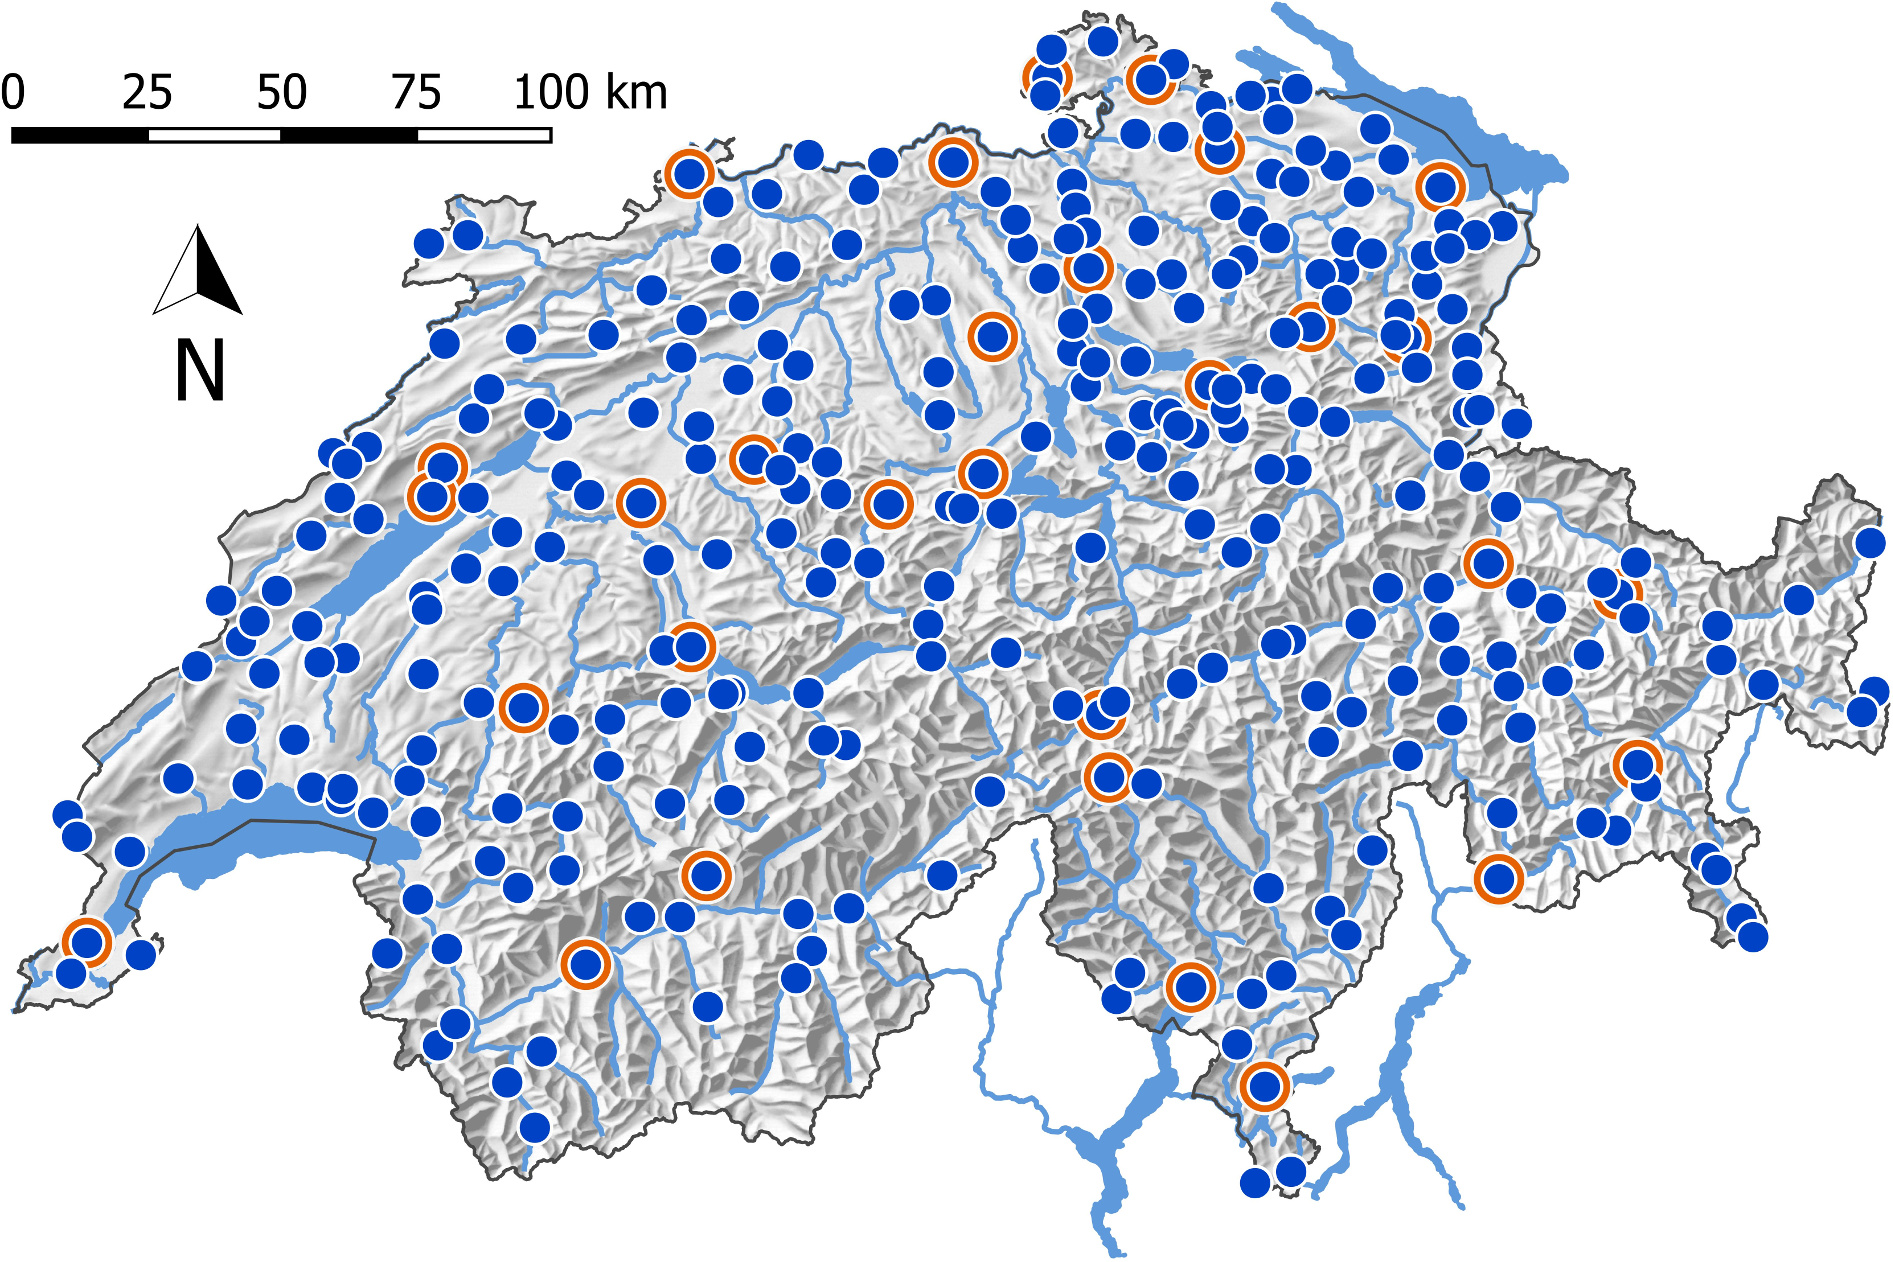
\includegraphics[width=19pc,angle=0]{figure01.pdf}\\
%\appendcaption{A1}{Caption here.}
%\end{figure}
%
% All appendix figures/tables should be placed in order AFTER the main figures/tables, i.e., tables, appendix tables, figures, appendix figures.
%
%%%%%%%%%%%%%%%%%%%%%%%%%%%%%%%%%%%%%%%%%%%%%%%%%%%%%%%%%%%%%%%%%%%%%
%  REFERENCES
%%%%%%%%%%%%%%%%%%%%%%%%%%%%%%%%%%%%%%%%%%%%%%%%%%%%%%%%%%%%%%%%%%%%%
% Make your BibTeX bibliography by using these commands:
\bibliographystyle{ametsoc2014}
\bibliography{../../../Biblio/Mendeley/Export/4_articles-2017_JCli_reanalysis}


%%%%%%%%%%%%%%%%%%%%%%%%%%%%%%%%%%%%%%%%%%%%%%%%%%%%%%%%%%%%%%%%%%%%%
%  TABLES
%%%%%%%%%%%%%%%%%%%%%%%%%%%%%%%%%%%%%%%%%%%%%%%%%%%%%%%%%%%%%%%%%%%%%
%% Enter tables at the end of the document, before figures.
%%
%
%\begin{table}[t]
%\caption{This is a sample table caption and table layout.  Enter as many tables as
%  necessary at the end of your manuscript. Table from Lorenz (1963).}\label{t1}
%\begin{center}
%\begin{tabular}{ccccrrcrc}
%\hline\hline
%$N$ & $X$ & $Y$ & $Z$\\
%\hline
% 0000 & 0000 & 0010 & 0000 \\
% 0005 & 0004 & 0012 & 0000 \\
% 0010 & 0009 & 0020 & 0000 \\
% 0015 & 0016 & 0036 & 0002 \\
% 0020 & 0030 & 0066 & 0007 \\
% 0025 & 0054 & 0115 & 0024 \\
%\hline
%\end{tabular}
%\end{center}
%\end{table}


\begin{table*}[t]
	\caption{Considered analogue methods with increasing complexity. P0 is the preselection (PC: on calendar basis, that is $\pm 60$ days around the target date), L1, L2 and L3 are the subsequent levels of analogy. The meteorological variables are: SLP -- mean sea level pressure, Z -- geopotential height, T -- air temperature, W -- vertical velocity, MI -- moisture index, which is the product of the relative humidity at the given pressure level and the total water column. The analogy criterion is S1 for SLP and Z and RMSE for the other variables.}
	\begin{center}
		\begin{tabular}{cccccl}
			\hline
			\textbf{Method} & \textbf{P0} & \textbf{L1} & \textbf{L2} & \textbf{L3} & \textbf{Reference} \\ 
			\hline 
			\multirow{2}{*}{\textbf{2SLP}} & \multirow{2}{*}{PC} & SLP@12h &&& \\
			&& SLP@24h &&& \\
			\hline 
			\multirow{2}{*}{\textbf{2Z}} & \multirow{2}{*}{PC} & Z1000@12h &&& \multirow{2}{*}{\citealt{Bontron2004}} \\
			 && Z500@24h &&& \\
	 		\hline 
			\multirow{4}{*}{\textbf{4Z}} & \multirow{4}{*}{PC} & Z1000@06h &&& \multirow{4}{*}{\citealt{Horton2017b}} \\
			 && Z1000@30h &&& \\
			 && Z700@24h &&& \\
			 && Z500@12h &&& \\
			\hline 
			\multirow{2}{*}{\textbf{2Z-2MI}} & \multirow{2}{*}{PC} & Z1000@12h & \multirow{2}{*}{MI850@12+24h} && \multirow{2}{*}{\citealt{Bontron2004}} \\
			&& Z500@24h &&& \\
			\hline 
			\multirow{4}{*}{\textbf{4Z-2MI}} & \multirow{4}{*}{PC} & Z1000@30h &&& \multirow{4}{*}{\citealt{Horton2017b}}\\
			&& Z850@12h & MI700@24h && \\
			&& Z700@24h & MI600@12h && \\
			&& Z400@12h &&& \\
			\hline 
			\multirow{2}{*}{\textbf{PT-2Z-4MI}} & T925@36h & Z1000@12h & MI925@12+24h && \multirow{2}{*}{\citealt{BenDaoud2016}} \\
			& T600@12h & Z500@24h & MI700@12+24h && \\
			\hline 
			\multirow{2}{*}{\textbf{PT-2Z-4W-4MI}} & T925@36h & Z1000@12h & \multirow{2}{*}{W850@06-24h} & MI925@12+24h & \multirow{2}{*}{\citealt{BenDaoud2016}} \\
			& T600@12h & Z500@24h && MI700@12+24h & \\
			\hline 
			
		\end{tabular} 
	\end{center}
	\label{table:methods}
\end{table*}



\begin{table*}[t]
	\caption{Assessed reanalysis datasets with their respective available period, timestep and resolution.}
	\begin{center}
		\begin{tabular}{cccccccc}
			\hline
			\multirow{2}{*}{\textbf{Id}} & \multirow{2}{*}{\textbf{Institutions}} & \multirow{2}{*}{\textbf{Name}} & \textbf{Period} & \textbf{Output} & \textbf{Model} & \textbf{Model} & \textbf{Assimilation}\\ 
			&&& \textbf{of record} & \textbf{resolution} & \textbf{resolution} & \textbf{vintage} & \textbf{technique} \\ 
			\hline 
			\textbf{NR-1} & NCEP, NCAR & Reanalysis I & 1948 -- present & 2.5\degree x 2.5\degree & T62 ($\sim$1.88\degree) & 1995 & 3D-Var\\
			\textbf{NR-2} & NCEP, DOE & Reanalysis II & 1948 -- present & 2.5\degree x 2.5\degree & T62 ($\sim$1.88\degree) & 2001 & 3D-Var\\
			\textbf{ERA-INT} & ECMWF & ERA-Interim & 1979 -- present & 0.75\degree x 0.75\degree & T255 ($\sim$0.70\degree) & 2006 & 4D-Var\\
			\textbf{CFSR} & NCEP & Clim. Forecast Sys. Rean. & 1979 -- present & 0.5\degree x 0.5\degree & T382 ($\sim$0.31\degree) & 2009 & 3D-Var\\
			\textbf{JRA-55}  & JMA & Japanese 55-year Rean. & 1958 -- 2015 & 1.25\degree x 1.25\degree & T319 ($\sim$0.36\degree) & 2009 & 4D-Var\\
			\textbf{JRA-55C}  & JMA & JRA-55 Conventional Data & 1958 -- 2015 & 1.25\degree x 1.25\degree & T319 ($\sim$0.36\degree) & 2009 & 4D-Var\\
			\textbf{20CR-2c} & NOAA-CIRES & 20th Century Rean. V2c & 1851 -- 2014 & 2\degree x 2\degree & T62 ($\sim$1.88\degree) & 2009 & E. K. filter\\
			\textbf{ERA-20C} & ECMWF & ERA 20th century & 1900 -- 2011 & 1\degree x 1\degree & T159 ($\sim$1.13\degree) & 2012 & 4D-Var\\
			\textbf{MERRA-2} & NASA & MERRA-2 & 1980 -- present & 0.625\degree x 0.5\degree & 0.625\degree x 0.5\degree & 2014 & 3D-Var\\
			\textbf{CERA-20C} & ECMWF & CERA-20C & 1901 -- 2010 & 1\degree x 1\degree & T159 ($\sim$1.13\degree) & 2016 & 4D-Var\\
			\hline 
		\end{tabular} 
	\end{center}
	\label{table:datasets}
\end{table*}







%%%%%%%%%%%%%%%%%%%%%%%%%%%%%%%%%%%%%%%%%%%%%%%%%%%%%%%%%%%%%%%%%%%%%
%  FIGURES
%%%%%%%%%%%%%%%%%%%%%%%%%%%%%%%%%%%%%%%%%%%%%%%%%%%%%%%%%%%%%%%%%%%%%
%% Enter figures at the end of the document, after tables.
%%
%
%\begin{figure}[t]
%  \noindent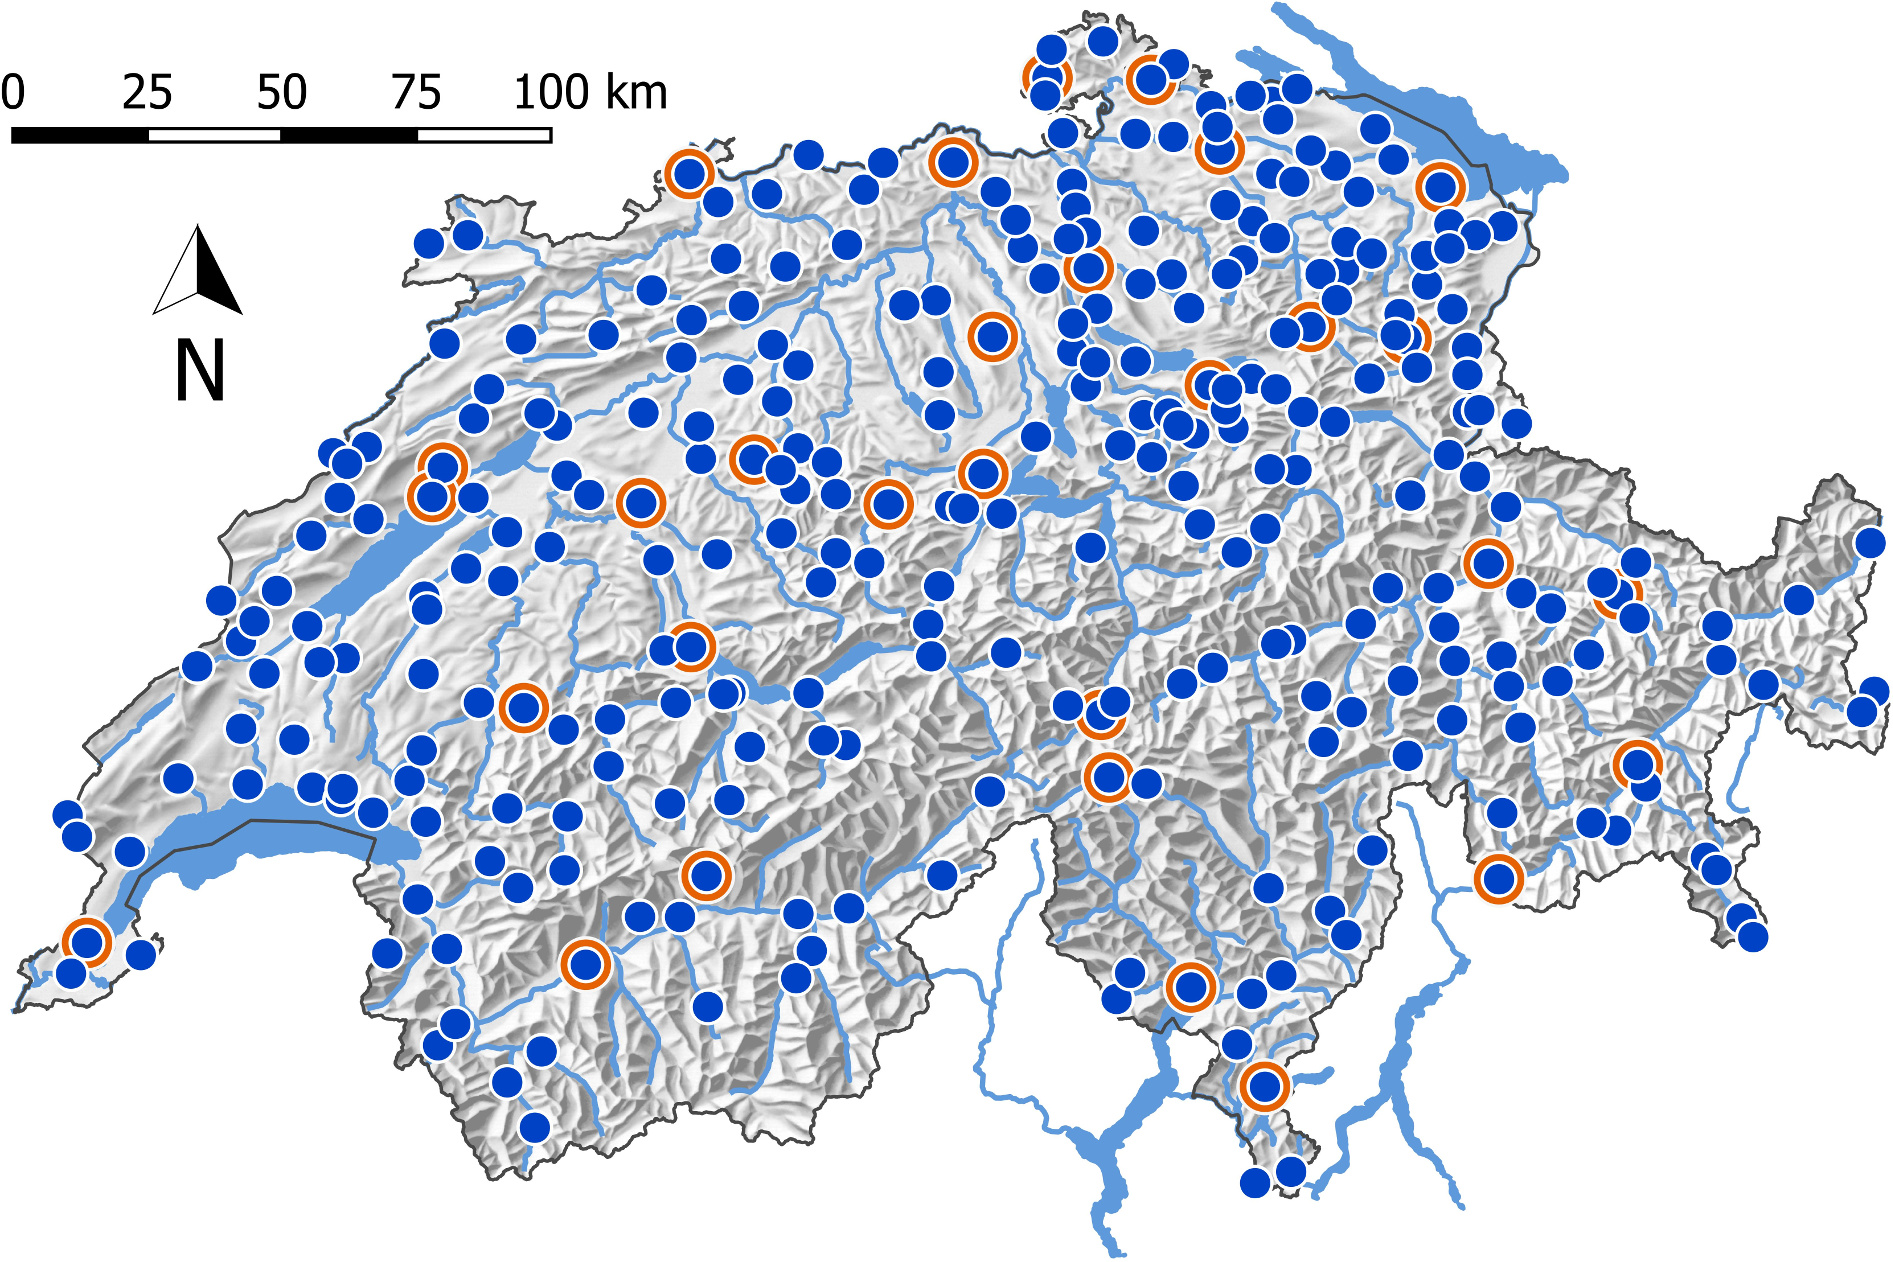
\includegraphics[width=19pc,angle=0]{figure01.pdf}\\
%  \caption{Enter the caption for your figure here.  Repeat as
%  necessary for each of your figures. Figure from \protect\cite{Knutti2008}.}\label{f1}
%\end{figure}

\begin{figure}[t]
  \noindent\includegraphics[width=19pc,angle=0]{figures/map-stations.jpg}\\
  \caption{Map of the 301 precipitation stations with a good data coverage of the period 1981--2010 (blue dots), and the 30 stations with long archives (orange).}
	\label{fig:stations}
\end{figure}

\begin{figure}[t]
	\noindent\includegraphics[width=39pc,angle=0]{figures/boxplot-all-methods-values.pdf}\\
	\caption{CRPSS score for all stations and for all considered AMs and reanalysis datasets. A higher CRPSS score means better performance. The parameters of the AMs were calibrated for every station, every dataset, and every method.}
	\label{fig:comparison_values}
\end{figure}

\begin{figure}[t]
	\noindent\includegraphics[width=39pc,angle=0]{figures/boxplot-all-methods-relative.pdf}\\
	\caption{Effect of the reanalysis dataset on the performance isolated by processing the improvement in CRPSS for one dataset compared to the mean performance on all datasets, per station and per method. Note that the methods cannot be compared here, only the datasets.}
	\label{fig:comparison_relative}
\end{figure}

\begin{figure}[t]
	\noindent\includegraphics[width=38pc,angle=0]{figures/maps-best-methods.pdf}\\
	\caption{Best method per station for the different datasets. NR-2 and JRA-55C are not shown as they are similar to NR-1 and JRA-55 respectively.}
	\label{fig:map_best_methods}
\end{figure}

\begin{figure}[t]
	\noindent\includegraphics[width=39pc,angle=0]{figures/boxplot-all-methods-relative-eq0.pdf}\\
	\caption{Same as Fig. \ref{fig:comparison_relative}, but for target days with no precipitation and expressed as a relative CRPSS. The methods cannot be compared here, only the datasets.}
	\label{fig:comparison_relative_P0}
\end{figure}

\begin{figure}[t]
	\noindent\includegraphics[width=39pc,angle=0]{figures/boxplot-all-methods-relative-q95.pdf}\\
	\caption{Same as Fig. \ref{fig:comparison_relative}, but for target days with precipitation above the all days 95th percentile and expressed as a relative CRPSS. The methods cannot be compared here, only the datasets.}
	\label{fig:comparison_relative_Pq95}
\end{figure}

\begin{figure}[t]
	\noindent\includegraphics[width=19pc,angle=0]{figures/similarities-analogue-dates.pdf}\\
	\caption{Percentage of similar analogue dates selected when using the reanalysis datasets in columns that are also found when using the datasets in rows for different AMs. The values are averaged for all stations on the VP.}
	\label{fig:similarities_analogue_dates}
\end{figure}

\begin{figure}[t]
	\noindent\includegraphics[width=19pc,angle=0]{figures/plot-impact-resolution-spread.pdf}\\
	\caption{Impact (difference in CRPSS) of a decrease in grid resolution (degrees) for different datasets and AMs on the CP. The line represents the median and the shaded area represents the first and the third quartiles (on 30 stations).}
	\label{fig:plot_impact_resolution}
\end{figure}

\begin{figure}[t]
	\noindent\includegraphics[width=19pc,angle=0]{figures/plot-impact-length-spread-CP.pdf}\\
	\caption{Impact (difference in CRPSS) of an increase in the archive length (years) for different datasets and AMs. Results for the 4Z method are displayed along with the 2Z method, but with dashed lines. The line represents the median and the shaded area represents the first and the third quartiles (on 30 stations).}
	\label{fig:plot_impact_length_CP}
\end{figure}

\begin{figure}[t]
	\noindent\includegraphics[width=19pc,angle=0]{figures/plot-impact-length-spread-VP.pdf}\\
	\caption{Same as Fig. \ref{fig:plot_impact_length_CP} but for the VP.}
	\label{fig:plot_impact_length_VP}
\end{figure}

\begin{figure}[t]
	\noindent\includegraphics[width=19pc,angle=0]{figures/plot-impact-members-2Z.pdf}\\
	\caption{Impact (difference in CRPSS) of an increase in the number of ensemble members used for the 2Z method and for CERA-20C and 20CR-2c datasets. The results are provided for two periods: (a, c) 1981--2010 and (b, d) 1901--1930. Two approaches were assessed: (a, b) the first allowing duplicate analogue dates ("w.d.d.") and (c, d) the second without duplicate analogue dates ("wo.d.d."). The line represents the median and the shaded area represents the first and the third quartiles (on 30 stations). The dashed line and striped area correspond to results on the VP. The 56 members of 20CR-2c were assessed and the tendencies continue, but the plots are split at 30 members.}
	\label{fig:plot_impact_members_2Z}
\end{figure}

\begin{figure}[t]
	\noindent\includegraphics[width=19pc,angle=0]{figures/plot-impact-members-2Z-2MI.pdf}\\
	\caption{Same as Fig. \ref{fig:plot_impact_members_2Z} but for the 2Z-2MI method.}
	\label{fig:plot_impact_members_2Z-2MI}
\end{figure}

\end{document}